\documentclass{article}
\usepackage[utf8]{inputenc} % Codificación del texto
\usepackage{amsmath} % Mejoras y más símbolos matemáticos
\usepackage{graphicx}

\begin{document}
	\begin{center}
		\Large \textbf{Las Leyes de Maxwell} \\
		\vspace{1em} % Espacio vertical
		\small 20 de abril de 2024
	\end{center}

	\begin{abstract}
		En este capítulo, exploraremos una de las piedras angulares de la física moderna: las ecuaciones de Maxwell. 
		Desarrolladas en la segunda mitad del siglo XIX por James Clerk Maxwell, estas ecuaciones revolucionaron nuestra comprensión de los fenómenos eléctricos y magnéticos, al unificarlos en un solo marco teórico. Maxwell demostró que la electricidad, el magnetismo y la luz son manifestaciones de un mismo fenómeno: el campo electromagnetico
	\end{abstract}
		
	
\section{La Ley de Gauss para el Campo Eléctrico}

La Ley de Gauss es una herramienta fundamental en el análisis de campos eléctricos en la electrostática, proporcionando un método eficiente para calcular el campo eléctrico en presencia de simetría. A continuación, desarrollamos la Ley de Gauss en el contexto de cargas puntuales y distribuciones de carga más complejas.

\subsection{Fundamentos Teóricos}
Consideremos una carga puntual \( Q \) ubicada en el origen. La ley de Gauss puede demostrarse utilizando una superficie esférica de radio \( r \) centrada en la carga.

\subsection{Campo Eléctrico de una Carga Puntual}
El campo eléctrico \( \mathbf{E} \) generado por una carga puntual en un punto en el espacio se define como:
\begin{equation}
	\mathbf{E} = \frac{Q}{4\pi \epsilon_0 r^2} \hat{r}
\end{equation}
donde \( \epsilon_0 \) es la permitividad del vacío, \( r \) es la distancia desde la carga al punto de interés, y \( \hat{r} \) es el vector unitario radial hacia fuera.

\subsection{Flujo Eléctrico}
El flujo eléctrico \( \Phi_E \) a través de la superficie esférica se calcula como el producto escalar del campo eléctrico y el área diferencial \( d\mathbf{A} \) sobre la superficie cerrada \( S \):
\begin{equation}
	\Phi_E = \oint_S \mathbf{E} \cdot d\mathbf{A}
\end{equation}
Donde \( d\mathbf{A} = r^2 \sin\theta d\theta d\phi \hat{r} \) para una esfera en coordenadas esféricas.

\subsection{Cálculo del Flujo}
Sustituyendo \( \mathbf{E} \) y \( d\mathbf{A} \) en la integral para \( \Phi_E \):
\begin{align}
	\Phi_E &= \oint_S \left( \frac{Q}{4\pi \epsilon_0 r^2} \hat{r} \right) \cdot (r^2 \sin\theta d\theta d\phi \hat{r}) \\
	&= \frac{Q}{4\pi \epsilon_0} \oint_S \sin\theta d\theta d\phi \\
	&= \frac{Q}{4\pi \epsilon_0} \cdot 4\pi \\
	&= \frac{Q}{\epsilon_0}
\end{align}
Asi la Ley de Gauss se expresa matemáticamente como:

\begin{equation}
	\oint_S \mathbf{E} \cdot d\mathbf{A} = \frac{Q_{\text{enc}}}{\epsilon_0}
\end{equation}

donde $\oint_S$ denota la integral sobre una superficie cerrada $S$, $\mathbf{E}$ es el campo eléctrico, $d\mathbf{A}$ es el vector área infinitesimal normal a la superficie, $Q_{\text{enc}}$ es la carga total encerrada por la superficie, y $\epsilon_0$ es la permitividad del vacío.

\subsection{Interpretación Física}

Esta ley establece que el flujo neto del campo eléctrico a través de cualquier superficie cerrada es igual a la carga neta encerrada por la superficie dividida por la permitividad del vacío. Esta propiedad es independiente de la forma de la superficie siempre que se encierre la misma carga.

\subsection{Aplicación a Geometrías Esféricas}

Consideremos una carga puntual $Q$ ubicada en el origen. Si elegimos una superficie esférica de radio $r$, centrada en la carga, el campo eléctrico en cualquier punto de esta superficie, debido a la simetría radial, es:

\begin{equation}
	E = \frac{Q}{4\pi \epsilon_0 r^2}
\end{equation}

El área de esta esfera es $4\pi r^2$. Por lo tanto, el flujo $\Phi_E$ a través de la superficie es:

\begin{equation}
	\Phi_E = E \cdot 4\pi r^2 = \frac{Q}{\epsilon_0}
\end{equation}

Este cálculo confirma la Ley de Gauss para una configuración simétrica donde el campo eléctrico y el vector área son paralelos en todos los puntos de la superficie.

\subsection{Generalizaciones y Limitaciones}

La Ley de Gauss es extremadamente útil en casos con alta simetría, como esferas, cilindros o planos. Sin embargo, su utilidad se reduce en situaciones sin simetría clara, donde puede ser más práctico utilizar directamente la ley de Coulomb combinada con el principio de superposición.

\section{Ley de Gauss para el Campo Magnético}
Esta ley afirma que el flujo magnético a través de una superficie cerrada es cero, implicando la no existencia de monopolos magnéticos
consideraremos el campo magnético generado por un dipolo magnético como un ejemplo práctico y calcularemos el flujo a través de una superficie cerrada que lo envuelve.

\subsection{Campo Magnético de un Dipolo}
El campo magnético \(\mathbf{B}\)producido por un dipolo magnético se expresa en términos de su momento magnético \(\mathbf{m}\)

 
y es dado por:
\begin{equation}
	\mathbf{B}(\mathbf{r}) = \frac{\mu_0}{4\pi} \frac{3(\mathbf{m} \cdot \hat{r})\hat{r} - \mathbf{m}}{r^3}
\end{equation}
donde \(\mathbf{r}\) es la posición relativa al dipolo, 
	\(\hat{r}\) es el vector unitario en la dirección de \(\mathbf{r}\),y\(r\) es la magnitud de \(\mathbf{r}\).

\subsection{Flujo Magnético a través de una Superficie Cerrada}
El flujo magnético \(\Phi_B\) a través de una superficie cerrada \(S\) se calcula como el producto escalar del campo magnético y el área diferencial \(d\mathbf{A}\) sobre la superficie:
\begin{equation}
	\Phi_B = \oint_S \mathbf{B} \cdot d\mathbf{A}
\end{equation}

\subsection{Evaluación del Flujo Magnético}
Debido a la naturaleza del campo magnético de un dipolo (o cualquier otra configuración real de campo magnético), que siempre tiene líneas de campo que entran y salen de la superficie cerrada sin fuentes o sumideros dentro de ella, el flujo neto es cero:
\begin{align}
	\Phi_B &= \oint_S \left(\frac{\mu_0}{4\pi} \frac{3(\mathbf{m} \cdot \hat{r})\hat{r} - \mathbf{m}}{r^3}\right) \cdot d\mathbf{A} \\
	&= 0
\end{align}
Este resultado se debe a que para cada línea de campo que entra en la superficie, hay una línea correspondiente que sale, cancelando así el flujo neto.

\section{Ley de Faraday}
La Ley de Faraday establece que la fuerza electromotriz inducida en cualquier circuito cerrado es igual a la tasa de cambio del flujo magnético a través del circuito. Matemáticamente, se expresa como:
\begin{equation}
	\mathcal{E} = -\frac{d\Phi_B}{dt}
\end{equation}
donde \(\mathcal{E}\) es la fuerza electromotriz inducida y \(\Phi_B\) es el flujo magnético. El signo negativo indica la dirección de la fuerza electromotriz y la corriente resultante, según la ley de Lenz.

\subsection{Experimento de Faraday}
El experimento ilustrativo de Faraday involucra un conductor en forma de espira moviéndose a través de un campo magnético. A medida que el conductor corta líneas de campo magnético, se induce una corriente eléctrica debido al cambio en el flujo magnético a través de la espira. 


\subsection{Aplicaciones}
Las aplicaciones de la inducción electromagnética son vastas, incluyendo la generación de electricidad en generadores eléctricos, transformadores y en la tecnología de sistemas de transporte como trenes magnéticos.


\section{Ley de Ampère-Maxwell}
Maxwell añadió un término a la ley de Ampère para incluir la corriente de desplazamiento, que es crucial para la conservación de la carga:
\begin{equation}
	\nabla \times \mathbf{B} = \mu_0 \mathbf{J} + \mu_0 \epsilon_0 \frac{\partial \mathbf{E}}{\partial t}
\end{equation}

\subsection{Importancia y Aplicaciones}
Las Ecuaciones de Maxwell no solo explican fenómenos eléctricos y magnéticos sino que también predicen la existencia de ondas electromagnéticas, un hallazgo que ha llevado a tecnologías revolucionarias como la radio, la televisión, y las telecomunicaciones.

%quizas aqui deba agregar la info sobre el vector Poynting

\section{El Vector Poynting y la Conservación de la Energía}
El vector Poynting, \(\mathbf{S}\), es fundamental para entender cómo la energía se transporta en los campos electromagnéticos. Representa la tasa de flujo de energía por unidad de área en un punto dado en el espacio y dirección.

\subsection{Definición del Vector Poynting}
El vector Poynting se define como el producto cruz entre los campos eléctrico y magnético:
\begin{equation}
	\mathbf{S} = \frac{1}{\mu_0} \mathbf{E} \times \mathbf{B}
\end{equation}
donde \(\mathbf{E}\) es el campo eléctrico, \(\mathbf{B}\) es el campo magnético, y \(\mu_0\) es la permeabilidad del vacío.

\subsection{Interpretación Física}
El vector Poynting describe la dirección y magnitud del flujo de energía electromagnética. Si \(\mathbf{S}\) es positivo, la energía fluye en la dirección de \(\mathbf{S}\); si es negativo, fluye en la dirección opuesta.

\subsection{Teorema de Poynting}
El teorema de Poynting es una declaración de la conservación de la energía para los campos electromagnéticos. Matemáticamente se expresa como:
\begin{equation}
	\nabla \cdot \mathbf{S} + \frac{\partial u}{\partial t} = -\mathbf{J} \cdot \mathbf{E}
\end{equation}
donde \(u\) es la densidad de energía del campo electromagnético, \(\mathbf{J}\) es la densidad de corriente eléctrica, y \(\mathbf{E}\) es el campo eléctrico. Este teorema indica que la disminución de la energía electromagnética en un volumen dado es igual al trabajo realizado por el campo sobre las cargas más la energía que fluye fuera del volumen.

\subsection{Aplicaciones del Vector Poynting}
El vector Poynting no solo es útil para calcular la potencia transmitida por las ondas electromagnéticas, sino que también es esencial en el diseño de antenas, en el estudio de la propagación de ondas de radio y en muchos otros aspectos de la ingeniería eléctrica y las telecomunicaciones.

\section{Leyes de Maxwell y Vector Poynting}
Las ecuaciones de Maxwell son el pilar del electromagnetismo clásico, describiendo cómo los campos eléctricos y magnéticos se propagan y afectan entre sí. Estas ecuaciones son esenciales para entender desde la radio hasta la luz visible.

\subsection{Formulación de las Ecuaciones de Maxwell}
Las Ecuaciones de Maxwell consisten en cuatro ecuaciones diferenciales que relacionan los campos eléctrico (\(\mathbf{E}\)) y magnético (\(\mathbf{B}\)) con las distribuciones de carga (\(\rho\)) y corriente (\(\mathbf{J}\)). 
	completando las ecuaciones, obtenidas experimentalmente
	
 	\begin{minipage}{.45\textwidth}
		\begin{equation*}
			\nabla\cdot\mathbf{\bar{E}} = 4 \pi \rho
		\end{equation*}
		\begin{equation*}
			\nabla\times\mathbf{\bar{E}} = -\frac{1}{c} \frac{\partial \mathbf{\bar{B}}}{\partial t}
		\end{equation*}
		\subsubsection*{Ecuaciones de Electroestatica}
	\end{minipage}%  % El comentario aquí es para evitar espacios adicionales
	\begin{minipage}{.45\textwidth}
		\begin{equation*}
			\nabla \cdot \mathbf{\bar{B}} = 0 \text{(1)}
		\end{equation*}
		\begin{equation*}
			\nabla \times \mathbf{\bar{B}} = \frac{4\pi}{c} \mathbf{\bar{J}}
		\end{equation*}
		\subsubsection*{Ecuaciones de Magnetostatica}
	\end{minipage}
	
	
	\subsection{Fuerza de Lorentz}
	\[
	\mathbf{\bar{F}} = q\mathbf{\bar{E}} + q\frac{\mathbf{\bar{v}}}{c} \times \mathbf{\bar{B}}
	\]
	
	y empleando la ecuacion de continuidad de carga obtenemos
	\begin{equation*}
		\frac{d\delta}{dt} + \nabla \cdot \mathbf{\bar{J}}=0  \text{(2)}
	\end{equation*}
	
	y resolviendo la incongruencia en \((1)\) donde
	\begin{equation*}
		\nabla(\nabla\times\mathbf{\bar{B}})=0=\frac{4\pi}{c}\nabla\mathbf{\bar{J}} \text{(2)}
	\end{equation*}
	
	mostrando incompatibilidad con \((2)\), lo cual permite manipular
	\begin{equation*}
			\nabla\times\mathbf{\bar{B}}=\frac{4\pi}{c} + \text{(*)}
	\end{equation*}
	donde \((*)\) es un termino aun desconocido
	
	para hallar \((*)\)) primero organizamos \((3)\) como 
	y resolviendo la incongruencia en \((1)\) donde
	\begin{equation*}
		\nabla(\nabla\times\mathbf{\bar{B}})=0=\frac{4\pi}{c} \nabla \mathbf{\bar{J}} + \nabla\text{(*)}
	\end{equation*}
	
	y aplicando la ecuacion de continuidad tenemos que 
	\begin{equation*}
		\frac{4\pi}{c} \frac{\partial d\delta}{\partial dt} = \nabla\cdot\text{(*)} \text{(4)}
	\end{equation*}
	
	una vez aqui, considerando que nuestras ecuaciones de electroestatica y magnetoestatica aun son validas, organizamos y obtenemos
	\begin{equation*}
		\frac{1}{c} \frac{\partial d}{\partial dt}\nabla \cdot \mathbf{\bar{E}}=\nabla \text{(*)}
	\end{equation*}
	
	si se quiere compatibilizar \((4)\) y \((5)\), agregamos algo que cumpla
	\begin{equation*}
		\frac{1}{c}\frac{\partial d}{\partial dt}\nabla\cdot\mathbf{\bar{E}}=\nabla(\frac{1}{c}\frac{\partial d}{\partial dt}\mathbf{\bar{E}})
	\end{equation*}
	Aqui es donde Maxwell propone que 
	\begin{equation*}
		\text{(*)}=\frac{1}{c}\frac{\partial d}{\partial dt}\bar{E
	\end{equation*}
	lo que hace que la ecuacion  \(\nabla \cdot \mathbf{B}\) sea igual a la ecuacion \(\nabla \cdot \mathbf{E}\), y asi obtenemos que
		\begin{minipage}{.5\textwidth}
		\begin{equation*}
			\nabla \cdot \mathbf{\bar{E}} = 4 \pi \rho
		\end{equation*}
		\begin{equation*}
			\nabla \times \mathbf{\bar{E}} = -\frac{1}{c} \frac{\partial \mathbf{\bar{B}}}{\partial t}
		\end{equation*}
	\end{minipage}%  % El comentario aquí es para evitar espacios adicionales
	\begin{minipage}{.5\textwidth}
		\begin{equation*}
			\nabla \cdot \mathbf{\bar{B}} = 0
		\end{equation*}
		\begin{equation*}
			\nabla \times \mathbf{\bar{B}} = \frac{4\pi}{c} \mathbf{\bar{J}}
		\end{equation*}
	\end{minipage}
	\[
	\mathbf{\bar{F}} = q\mathbf{\bar{E}} + q\frac{\bar{v}}{c} \times \mathbf{\bar{B}}
	\]	
	Donde la nueva \(\nabla \times \mathbf{\bar{B}}\)sera la ecuacion de Ampere-Maxwell, completando asi las ecuaciones de Maxwell, un sistema completo y compatible entre si.	
	Donde se incluye la ecuacion de continuidad, que puede ordenarse como
	\begin{equation}
		0=\frac{4\pi}{c}\nabla\cdot\bar{J}+\frac{4\pi}{c}\frac{\partial}{\partial dt}\delta
	\end{equation}
	Si consideramos que en el vacio
	\begin{minipage}{.5\textwidth}
		\begin{equation*}
			\nabla \cdot \mathbf{\bar{E}} = 0
		\end{equation*}
		\begin{equation*}
			\nabla \times \mathbf{\bar{E}} = -\frac{1}{c} \frac{\partial \mathbf{\bar{B}}}{\partial t}
		\end{equation*}
	\end{minipage}%  % El comentario aquí es para evitar espacios adicionales
	\begin{minipage}{.5\textwidth}
		\begin{equation*}
			\nabla \cdot \mathbf{\bar{B}} = 0
		\end{equation*}
		\begin{equation*}
			\nabla \times \mathbf{\bar{B}} = \frac{1}{c} \frac{\partial \mathbf{\bar{E}}}{\partial t}
		\end{equation*}
	\end{minipage}
	donde 
	\begin{equation*}
		\nabla \mathbf{\bar{E}},\mathbf{\bar{B}}\neq0
	\end{equation*}
	Vemos que ante condiciones iniciales, se generara un campo magnetico que extraera la variable tiempo	
	\subsection{Problema sencillo}
	\begin{figure}[h]
		\centering 
		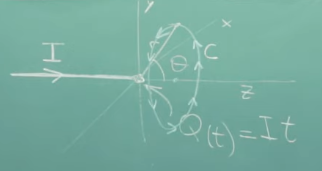
\includegraphics[width=0.5\textwidth]{imagen.png} % Cambia 'nombre_de_la_imagen.ext' por el nombre real de tu archivo y su extensión.
		\label{fig:mi_imagen} 
	\end{figure}	
	Calculando....
	\begin{equation*}
		\bar(E)(\bar(r),t)= \frac{Q(t)\hat{r}{r^2}=\frac{Q(t)\hat{I*t}{r^2}\hat{r}
	\end{equation*}
		\begin{equation*}
				B_{0}(r, \theta) \hat{y}
		\end{equation*}
		\begin{equation*}
				\oint_{C} \hat{B}*d\\hat{e} = \int_{S} (\nabla x \bar{B})\hat{n} ds=\int_{s} (\frac{4 \pi}{c} + \frac{1}}{c} \frac{\partial \mathbf{\bar{E}}}{\partial t}) \hat{n} ds
		\end{equation*}
		donde c es 0 y \(B*d\\hat{e} -> 2 \pi B_{0} \sin(\theta)\), asi
		\begin{equation*}
			2 \pi B_{0} \sin(\theta)= \frac{\partial}{\partial T}(\frac{7t}{r^2})(2\pi (1-\cos(\theta)))r^2 = \frac{1}{c}2\pi I(1-\cos(\theta))
		\end{equation*}
		\begin{equation*}
			B_{0}=\frac{1}{rc} * \frac{(1-\cos(\theta))}{\sin(\theta)}
		\end{equation*}
		Con las dos formas anteriores de los campos Eo, (\(\bar{B}\)) y usando er valor Bo hallado, verificamos que satisface las 4 ecuaciones de Maxwell		
		\subsection{Energia de campo E.M}
		\begin{figure}[h]
			\centering 
			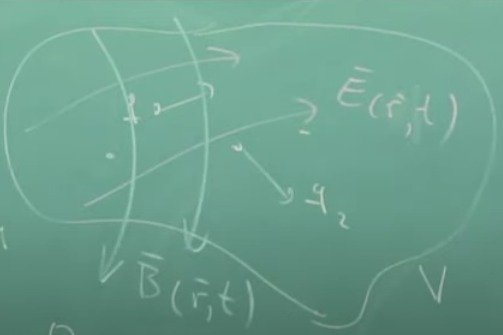
\includegraphics[width=0.5\textwidth]{imagen1.jpg}
			\label{fig:mi_imagen2} 
		\end{figure}
		Se tienen ciertas cargas que se mueven y generan campos electricos (magneticos)
		\begin{equation*}
			U total (conservada)= \text{U}_{mec} + \text{U}_(E.M)
		\end{equation*}
		\begin{equation*}
			\rho t -> \rho \text{U}_{\text{mec}} + \rho \text{U}_{\text{E.M}} + (\text{energia que sale del volumen} en \rho_{t}) =0		
		\end{equation*}
		\begin{equation*}
			\sum_{\alpha} \hat{F}_{\alpha} \rho_{\bar{r}\alpha}= \sum_{\alpha} \bar{F}_{\alpha} * \bar{V}_{\alpha}= \sum_{\alpha} (q_{\alpha} \bar{E} + \frac{q\alpha}{c} \bar{V}_{\alpha}x\bar{B})*\bar{V}_{\alpha} \rho t
		\end{equation*}
		\begin{equation*}
			\sum{\alpha} (q\alpha \bar{V}_{\alpha})*\bar{E} \rho t= \int{V} \bar{J} *\bar{E} d\r^3 dt
		\end{equation*}
		\begin{equation*}
			= \int{v} \bar{J}*\bar{E} dr^3 dt
		\end{equation*}		
		\begin{equation*}
			\frac{\rho_{Umec}{\rho_{t}}=\int{v} dr^3 \bar{\partial E}
		\end{equation*}
		Si usamos la ecuacion de Maxwell
		\begin{equation*}
			\bar{J}\bar{E} = (-\frac{1}{4\pi}+\frac{\rho_{\bar{E} {\rho_{t}
		\end{equation*}
		\begin{equation*}
			-\frac{1}{4\pi}\bar{E}\frac{\rho_{\bar{E}}}{\rho_{t}}  + \frac{c}{4\pi}(- \nabla (\bar{E}x\bar{B})+ \bar{B}*(\nabla x \bar{E}))
		\end{equation*}
		\begin{equation*}
			= -\frac{1}{4\pi}\bar{E}\frac{\rho_{\bar{E}}}{\rho_{t}} -\frac{1}{4\pi}\bar{B}\frac{d\bar{B}}{dt}-\frac{c}{4\pi}\nabla(\bar{E}x\bar{B})
		\end{equation*}
		donde \(\frac{d\bar{B}}{dt}\) fue planteado por Faraday
		\begin{equation}
			\frac{\partial U_{\text{mec}}}{\partial t} = - \int_{v} d^3r \left( \frac{\partial |E|^2}{\partial t} \cdot \frac{\partial |B|^2}{\partial t} \right) - \frac{c}{4\pi} \int d^3r \, \nabla \cdot \left( \bar{E} \times \bar{B} \right)			
		\end{equation}
		\begin{equation*}
			U_{\text{EM}}= \int d^3v \frac{E^2 +B^2}{8\pi}
		\end{equation*}		
		La energia que sale de V por unidad de tiempo
		\begin{equation*}
			\oint \frac{c}{4\pi}(\bar{E}\times\bar{B})\hat{n}ds
		\end{equation*}		
		A la anterior le suele llamar vector de Poynting \(\bar{S}\)
		donde
		\begin{equation}
			\bar{S}=\frac{c}{4\pi}(\bar{E}\times\bar{B})= \oint \bar{S}\hat{n}ds \text{vector flujo de energia}
		\end{equation}	
		\subsection{Ejemplos para entender el vector Poynting}
		Pensar en el vector ayuda a saber porque o en que caso tiene que aparecer o no algun campo para justificar los flujos de energia
		\begin{figure}[h]
			\centering 
			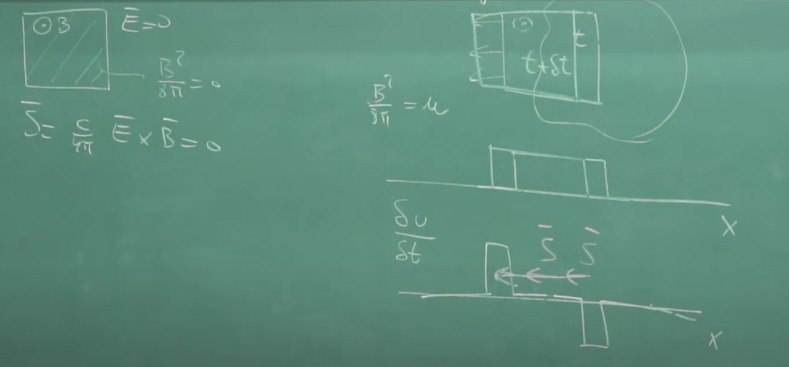
\includegraphics[width=0.5\textwidth]{imagen2.jpg}
			\label{fig:mi_imagen3} 
		\end{figure}
		Tambien se pueden generar paradojas
		\begin{figure}[h]
			\centering 
			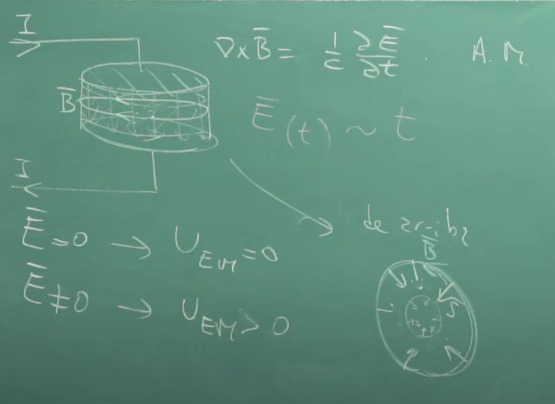
\includegraphics[width=0.5\textwidth]{imagen3.jpg}
			\label{fig:mi_imagen4} 
		\end{figure}
\end{document}
